\section{Introduction}

Statistical methods for analyzing network data have become increasingly useful for studying  phenomenon ranging from people communicating online to protein interactions \cite{Goldenberg2009}.
Stochastic blockmodels \cite{Nowicki2001, Kemp, Ishiguro2010} are a class of statistical models for static network data that employ latent variables to model unobserved heterogeneity by 1) assuming each node in the network belongs to some block (or cluster) and 2) parameterizing the probability of edges between nodes of each block.  % Such approaches are especially useful for large-scale network data where higher-order dependencies can cause models such as exponential random graph models to be too complex to fit.
% TODO: Cite Rodriguez: Modeling dynamics of social networks via h. blockmodels

Network data, however, is often collected as a sequence of events occurring over time.
Recent work leverages  continuous-time models from event history analysis  \cite{AalenOddO.2008} to model network-based event data \cite{Butts2008,Brandes2009,Perry2011,Stadtfeld2010,Stadtfeld2011,Opsahl2011,Vu2011,Vu2011a}.
These models allow one to specify how the process depends on the previous history of events.
In this way one may investigate theories about the underlying processes and make predictions about future data conditioned on the past.

A limitation of all of these approaches is the assumption of a single common behavior for all individuals.
In contrast, in real-world networks it is reasonable to expect {\it heterogeneity} in dynamic behavior.  
In an organization, the manner in which an individual communicates with others may be a function of an individual's {\it role} in the organization.
For example, in a university,  email communication patterns over time between professors, students, and staff will likely be quite different within and between the three groups.
%PS: not totally happy with this example since the "roles" are completely determined by one's "job title" and I think we would prefer something
% less explicit, e.g., that there are "leaders", "followers", etc, that go beyond just job titles. So feel free to edit this further!

%
%comprised of several teams, each team may uncover different patterns for collaborating via email---individuals in one group may respond more quickly, while another group may preferentially send to highly active individuals.

% TODO: Mention dynamic stochastic equivalence

% TODO: Incorporate notes from joint meeting:
% - used to thinking about actors differentiated by rates
% - other things in the dynamics than rates, e.g. form of interaction.
% - Also important aspect of modeling social dynamics.
% especially important in cases like plot 1(c) where classical methods
% will fail.

\begin{figure}
\centering
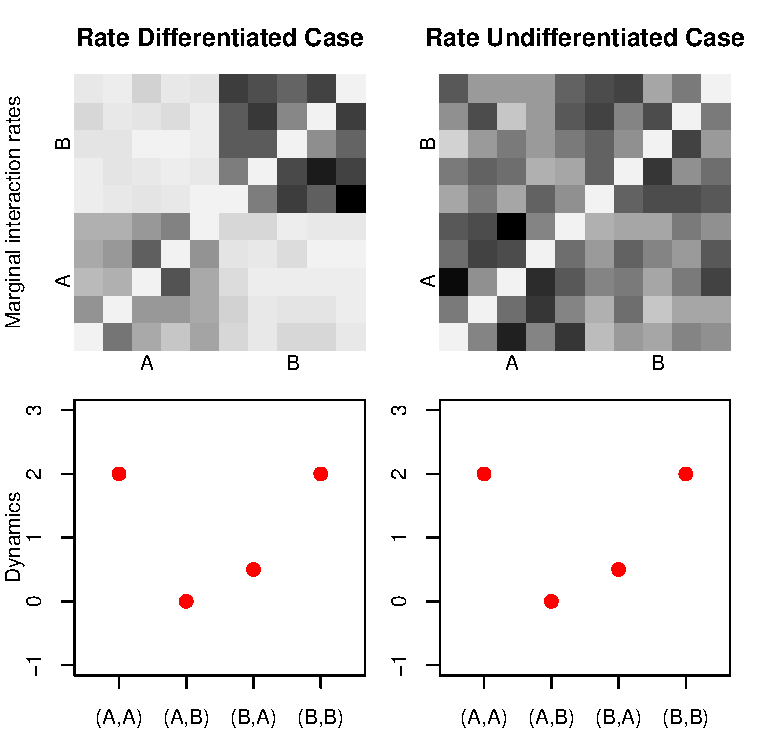
\includegraphics[scale=.8]{../figs/introexample/all}
% \begin{subfigure}[b]{0.45\textwidth}
% \centering
% \includegraphics[scale=.5]{../figs/introexample/mat1}
% \end{subfigure}
% ~
% \begin{subfigure}[b]{0.45\textwidth}
% \centering
% \includegraphics[scale=.5]{../figs/introexample/mat2}
% \end{subfigure}\\
% \begin{subfigure}[b]{0.45\textwidth}
% \centering
% \includegraphics[scale=.5]{../figs/introexample/dynamics1}
% \end{subfigure}
% ~
% \begin{subfigure}[b]{0.45\textwidth}
% \centering
% \includegraphics[scale=.5]{../figs/introexample/dynamics2}
% \end{subfigure}
\caption{}
\label{fig:example}
\end{figure}

Borrowing from the intuition of stochastic blockmodels, we propose a hierarchical model of continuous time network data to capture node-level heterogeneity, where we assume that latent clusters of nodes share similar patterns of interaction.
We describe parameter estimation and learning of  latent cluster assignments via MCMC, and illustrate the behavior of the model  with simulated data.
Using several real-world social network data sets involving dyadic communication, we compare the predictive performance of the fitted models to standard baselines.
Finally we show that the parameter estimates exhibit an interpretable structure to the event dynamics, allowing identification of particular \emph{roles} in communication.
